%!TEX root = ../thesis.tex
%*******************************************************************************
%****************************** Third Chapter **********************************
%*******************************************************************************
\chapter{Requirements Elicitation}
\graphicspath{{Chapter4/Figs/Raster/}{Chapter4/Figs/}}

Background literature review in Chapter 2.1 and 2.2 has driven the direction of the project and 
provided many of the functional requirements. This chapter describes the further collection of primary 
data, and provides the list of formal user requirements.

\section{Primary Data and Analysis}
Collecting primary data from shareholders of higher education e-learning systems would be able to:
\begin{itemize}
    \item reaffirm and further develop requirements obtained from literature
    \item obtain further requirements from real world painpoints and goals
\end{itemize}

\subsection{Methodology}

[TODO]

Method: qualitative

Instrument: Why interviews?

Sample: Participants are needed who are 
\begin{itemize}
    \item Teaching staff in higher education with 10+ years of experience
    \item Student
\end{itemize}Teachers with  in Who are they? Why? Convenience Sampling. Limitation: all CS department.

An ethics submission was completed on BREO and approval granted on 21st November. 
See Appendix (TODO) for the approved participant information sheet, consent form and example questions.

A total of five interviews were conducted between December 2017 and February 2018: 
two with teaching staff and three with student representatives. See table 
\ref{table:participants-req} for a more detailed description of these participants.

\begin{table}[!h] 
    \caption{Participants in primary data collection interviews}
    \centering
    \label{table:participants-req}
    \begin{tabularx}{\textwidth}{>{\bfseries}lX}
        Participant & Characterisation\\
        \toprule
        Educator A & lecturer in higher education for over 20 years, and an experienced higher education 
        administrator\\\midrule
        Educator B & lecturer in higher education for over 20 years, with research interests 
        in e-learning interactions, effectiveness and acceptance\\\midrule
        Student C & a university course representative for 3 years, which involves collecting and 
        communicating student feedback and attending staff-student liaison meetings \\\midrule
        Student D & a university peer assisted learning leader for 2 years, helping out lower level 
        students with their academic work by facilitating peer discussions, and escalating common problems
        to academic staff in debrief sessions\\\midrule
        Student E & a university course representative for 2 years and a peer assisted learning leader 
        for 1 year\\\bottomrule
    \end{tabularx}
\end{table}

\subsection{Interview Results and Analysis}

The raw data from interviews (transcripts) were contextually analysed and grouped into problem statements (PS), 
these problem statements were then sorted into groups to produce an affinity diagram (See figure 
\ref{fig:ps-affinity}).

Below you will find the sample questions asked for each group, detailed descriptions and relevant transcript 
snippets for each problem statements. 
Any specifics regarding course, staff and event details have been anonymised.

\begin{figure}[!ht] 
    \centering    
    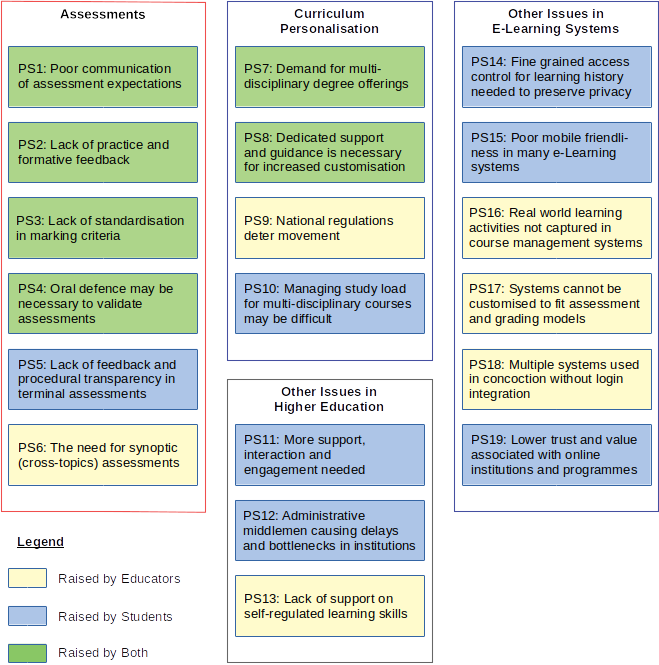
\includegraphics[width=1.0\textwidth]{ps-affinity}
    \caption[Affinity diagram for primary data]
        {Affinity diagram for problem statements devised from primary data}
    \label{fig:ps-affinity}
\end{figure}

\subsubsection{\underline{On Assessments}}

Sample Question: What are the problems with assessments in higher education today? / 
Is there tension between students and teachers over assessments, and why? 
\vspace{0.25cm}\\
\textbf{PS1: Poor communication of assessment expectations}\\
Four participants confirmed that the problem with transparency in expectations for 
assessments (as described in Chapter 2.1.1) does exist.\\
\textit{Educator B}: "Often it is not clear to the students what they have to do... staff [should be] 
making sure that it is clear what is expected of an assessment."\\
\textit{Student C}: "Sometimes [assessments] are unfair because they are based on things you have 
not learnt in lectures but have to read around... so not knowing what is actually assessed..." \\
\textit{Student D}: "Students have a lot of problem understanding what to do in assessments, it is not clear enough 
how you can prepare for it."\\
\textit{Student E}: "[Teachers] did not put it out clearly... all of the students where just lost on what 
they are expecting from our coursework... people feel too stupid to ask those questions."
\vspace{0.25cm}\\
\textbf{PS2: Lack of practice and formative feedback}\\
Students transitioning from school to higher education would experience a drop in formative assessments
(that do not affect their final grade) such as homework practices.\\
\textit{Educator B}: "[Students] are not used to not practising what they have to do over and over again 
before [assessments]... and that's what they had done at school... and the students that I feel most need 
formative feedback also tends not to do them."\\
\textit{Student D}: "[Students] really like past papers... Practice really helps... they are the best 
way of understanding what's coming in the exams."
\vspace{0.25cm}\\
\textbf{PS3: Lack of standardisation in marking criteria and lack of automation in module review}\\
\textit{Educator B}: "In [our department] we have those assessment forms that we have to fill in, 
which ensures we at least but something for each of the [marking criteria] boxes... the marking scheme 
is sent to the module reviewer, who reads them and ensures they are clear. This is all manual... 
We are one of the few departments in the university that has anything like this. In lot of departments, 
these are not clearly defined by a long stretch."\\
\textit{Student C}: "Having the marking criteria set in stone is actually the most important thing 
to students."
\textit{Student E}: "[Assessments] are kind of fair, but it depends on who your tutor is... 
some tutors were giving As out way too easily... there should have been some sort of structure that 
the tutors followed."
\vspace{0.25cm}\\
\textbf{PS4: Oral defence may be necessary to validate assessments}\\
\textit{Educator A}: "[Automated assessment] is problematic... to verify that is the viva (oral defence).
When I talk to my group and ask what they got from that [automated] test they said they got 100... 
but when I ask them to explain it to me, they could not. So the final piece of validation that is needed
before they move on from the level is to be able to question them on their answers. You can trust 
what's in the system but whether you trust the value of what's in a system depends on the viva."\\
\textit{Student E}: "Some people that I know faked a whole coursework yet still got a banging grade 
even though they did not produce any [of their work]... no one is checking properly."
\vspace{0.25cm}\\
\textbf{PS5: Lack of feedback and procedural transparency in terminal assessments}\\
\textit{Student C}: "One of the biggest issues is when you come out of the exams and you find out 
just the grade but you don't get to see the paper."
\vspace{0.25cm}\\
\textbf{PS6: The need for synoptic (cross-topics) assessments}\\
% Cross-curricular assessments here means assessing knowledge in multiple subjects in one 
% project or portfolio so as to promote learning that integrates knowledge across subjects.\\
\textit{Educator B}: "Assessments are very compartmentalised into their modules... that every module has 
its own assessments. This leads to students thinking that their learning in one module is irrelevant 
to another, whereas in the real world we draw knowledge from different areas."

\subsubsection{\underline{On Curriculum Personalisation}}

Sample Question: What do you think are the current road blocks to offering more multi-disciplinary, 
personalised, or even multi-institutional arrangements for higher education?
\vspace{0.25cm}\\
\textbf{PS7: There is a demand for multi-disciplinary degree offerings but only a few 
universities are capable of offering them}\\
It was argued by \textit{Educator B} that having the freedom to choose is better than universities 
defining programmes that encompasses two particular fields, because these defined degrees could have 
a low intake and not be economically viable. However, universities today seem to struggle with bureaucracy 
with students who wish to choose modules outside of their programme.\\
\textit{Educator B}: "Yes I do think there is a demand [for more multi-disciplinary offerings] and I know 
a lot of models that do work like this. The Open University and Oxford Brookes University do these 
style of degrees where students have some core modules that they have to do... surrounding that 
they can choose modules that then add up to a certain number of credits." \\
\textit{Student C}: "Definitely if there is a bit more combination, or an allowance in terms of 
picking [modules] for your degree... I think there is definitely a demand."\\
\textit{Student D}: "There is a range of students that you have to try and please...
I did hear one complaint... they didn't understand how [one module] has anything to do with the course, 
that it wasn't that hands-on and practical. I [thought] it was really good personally."
\vspace{0.25cm}\\
\textbf{PS8: Dedicated support and guidance is necessary for increased customisation}\\
There are careers that require multi-disciplinary backgrounds, but there is a risk of 
students not making informed choices.\\
\textit{Educator B}: "I think students need to be carefully guided through their choices and 
have good career advice... For example, the pharmaceutical industry is having a hard time 
finding people with a background in both IT and biology."\\
\textit{Student E}: "There is no point if it is like doing two half degrees and they are missing out."
\vspace{0.25cm}\\
\textbf{PS9: National regulations requiring programme outcomes and specifications deter movement}\\
The UK higher education academic infrastructure requires all degree programme to lay out 
programme outcomes and programme specifications, which makes movement difficult.\\
\textit{Educator A}: "If you want to move from [one institution] to somewhere else and you have 240 credits, 
the first thing I am going to ask you is, have you read my level 1 and level 2 outcomes? Are you 
in a place where you can, if you do level 3, meet the outcomes of the programme? ... 
[Our] credit model is not the same as the North American one, so actually movement 
between [institutions or programmes], despite the government always saying they want this, 
is mitigated against by the way we conceive education, which is about programmes representing... 
what you can do when you leave a programme."
% \textit{Educator A}: "You could radically liberalise it by having a set of terminal assessments that evaluate 
% whether a student satisfy the programme outcomes"\\
\vspace{0.25cm}\\
\textbf{PS10: Managing study load for multi-disciplinary courses may be difficult}\\
\textit{Student E}: "I don't think we have the time [to study many disciplines at once]... unless 
we have fewer modules... so their credits should be the same, they shouldn't take more credits 
because they chose to do another course."

\subsubsection{\underline{Other Issues in Higher Education}}

Sample Questions: What else needs improving in higher education in general?
\vspace{0.25cm}\\
\textbf{PS11: More support, interaction and engagement needed}\\
\textit{Student D}: "The way [teachers] interact sometimes is not that engaging... [they] could be 
giving out facts and information but they are not telling you... the interaction needs to be 
there... a lot of students would just come out [thinking] I don't understand what's just been said."\\
\textit{Student D}: "The contact time students and tutors have is not always as good as we think it is...
face to face contact, that's what students are not getting enough of... the support you get can really 
change the outcome of assessments."\\
\textit{Student E}: "Some students need a bit more help than others. Some people are embarrassed to 
face their learning difficulties."
\vspace{0.25cm}\\
\textbf{PS12: Administrative middlemen causing delays and bottlenecks in institutions}\\
\textit{Student E} has complained that feedback was not given on time to students, and the excuse 
given was that the teaching staff has sent the feedback to administrative staff but it takes time for 
them to upload it onto respective systems.
\vspace{0.25cm}\\
\textbf{PS13: Lack of support on self-regulated learning skills}\\
\textit{Educator B}: "[Students] don't realise the difference between school and university... the way 
they will be expected to learn... they have to do a lot of self-motivated learning and a lot of them 
find that a huge challenge. There is not enough help and guidance for students to make that transition."

\subsubsection{\underline{Other Issues in E-Learning Systems}}

Sample Questions: What other features would you like to see in a future e-Learning system for 
higher education?
\vspace{0.25cm}\\
\textbf{PS14: Fine grained access control for learning history needed to preserve privacy}\\
\textit{Student D}: "I don't think it's a good idea for all the records to be available to the public, 
not just anyone... I think students are very private... perhaps [the student could] allow employees and 
other institutions to view it."\\
\textit{Student E} expressed concern over aggregated data, such as gender comparisons and class rankings, 
arguing that institutions do not have rights to disclose that data without permission.
\vspace{0.25cm}\\
\textbf{PS15: Poor mobile friendliness in many e-Learning systems}\\
\textit{Student C} has pointed out that any new system should be built to be responsive and mobile friendly.
\vspace{0.25cm}\\
\textbf{PS16: Real world learning activities not captured in course management systems}\\
\textit{Educator A}: "There will be things that were part of the education experience that are outside of the system
such as face to face contact."
\vspace{0.25cm}\\
\textbf{PS17: Systems cannot be customised to fit assessment and grading models}\\
Many of the assessment features and functions on e-learning systems are incompatible 
with institutional requirements, or even national requirements. \textit{Educator A} pointed out how there is 
no global standard in grade point averages, and gave examples of staff:
\begin{itemize}
    \setlength\itemsep{0em}
    \item taking assessments outside the system, then putting the results back in
    \item mapping grades from a system using North American points (back to British grades)
    \item incorporating an extra viva (oral defence) assessment step outside of e-learning systems
    \item modifying a Scandinavian system that requires double marking for all assessments 
    to making double marking optional
\end{itemize}
\textbf{PS18: Multiple systems used in concoction without login integration}\\
\textit{Educator B}: "[Teachers] have to log into all of them separately... which I find frustrating. 
Students find it frustrating as well... Blackboard Learn [a course management system] is one set of 
software, their intranet is another, Wiseflow [an e-Assessment system] is another, another login system 
entirely for e-Vision [a student record system]. Usability becomes a major pain point."
\vspace{0.25cm}\\
\textbf{PS19: Lower trust and value associated with online institutions and programmes}\\
\textit{Student C}: "People tend to think online learning is a lot easier and it is devalued straight away. 
When you come to a campus to do it... it would probably be the same process as an online course but 
it would have more value because of the institution having a physical existence and not just a digital one."

% \textbf{- Allowing multiple forms of assessment for the same level of higher education qualification}\\
% Similar to how you could choose between the exam-oriented A-Levels or the portfolio-oriented BTEC diplomas 
% as a school leaving qualification in the UK.\\
% \textit{Student C}: "Some people are good in exams and some people prefer coursework... but you could 
% argue is it a good idea to give students that choice? Everyone will be happy... but from the institution's 
% point of view, you need to know what [standards] you get out there... it should be fair for everyone."
% \vspace{0.25cm}\\
% \textbf{- Lack of student demand for geographical movement}\\
% \textit{Educator A}: "People like the idea of choice... but there is no evidence that there is an appetite 
% from students for this. If I offer the whole cohort the option to do a year in another country,
% very few of them will take it up... it has to do with the British psyche of going to one place for 
% university."
% \vspace{0.25cm}\\
% \textit{Student C}: "Yes, students don't like assessments. Our [student union] vice-president is trying to 
% cut down the number of exams there are, converting them into courseworks."
% \textit{Student C}: "It wouldn't reduce the tension but would give people less of an excuse"

\section{Formal Requirements}

Table \ref{table:fx-reqs} lists out the functional requirements (FR) adopted by this 
project going forward. They are related to one or more of the problem statements (PS) gathered 
above from primary data, or to the literature reviewed in Chapter 2. 

Table \ref{table:nonfx-reqs} lists the non-functional requirements (NR) adopted by this 
project going forward. They are related to one or more of the problem statements (PS) gathered, 
or to usability heuristics.

These requirements have been ranked with the MoSCoW prioritisation
framework, which specified four levels of priority: Must Have, Should Have, Could Have, and Won’t Have 
this time \citep{agile2018moscow}. The MoSCoW levels are given from mainly a system engineering perspective 
in planning the minimum viable product for the demonstrator of this project, 
and do not necessarily reflect the priorities of the stakeholders.

\begin{table}[!h] 
    \caption{Prioritised list of functional requirements for this project}
    \centering
    \label{table:fx-reqs}
    \begin{tabularx}{\textwidth}{>{\bfseries}l>{\hsize=1.5\hsize}X>{\hsize=.5\hsize}Xl}
        & Requirement Statements & Related To & MoSCoW\\
        \toprule
        FR1 & The system would store learner records on a blockchain 
        & Ch 2.2.1 (LTSA) & Must Have
        \\\midrule
        FR2 & Teachers would be able to create and edit learning resources
        & Ch 2.2.1 (LTSA) & Must Have
        \\\midrule
        FR3 & Teachers would be able to create and edit assessments
        & Ch 2.2.1 (LTSA) & Must Have
        \\\midrule
        FR4 & The system would enforce the provision of learning outcomes, knowledge required 
        and assessment goals at the creation or update of modules & Ch 2.1.1 (Transparency), 
        PS1 & Must Have
        \\\midrule
        FR5 & The system would enforce predefined assessments rules (eg. marking schemes, 
        transparent procedures and feedback) with smart contracts 
        & Ch 2.1.1 (Transparency), PS3, PS5 & Must Have
        \\\midrule
        FR6 & The system would allow teachers to configure multiple assessments and 
        formative assessments for modules & PS2 & Could Have
        \\\midrule
        FR7 & The system would require vivas (oral defences) after automated assessments & 
        PS4 & Could Have
        \\\midrule
        FR8 & The system would provide flexible configurability for grade schema & PS17
        & Could Have
        \\\midrule
        FR9 & Teachers would be able to create a customised list of courses 
        for a student, customising programme outcomes and specifications 
        & Ch 2.1.2 (Personalisation), PS7, PS9 & Must Have
        \\\midrule
        FR10 & The system should feature dedicated support channels between students, teachers 
        and other advisors 
        & PS8, PS11 & Should Have
        \\\midrule
        FR11 & Students would be able to add assessment submissions on the blockchain 
        & Figure \ref{fig:moocon_assess} (Concept)& Must Have
        \\\midrule
        FR12 & The system would be able to generate certificates on the blockchain when a course 
        has been completed & Figure \ref{fig:moocon_assess} (Concept) & Must Have
        \\\midrule
        FR13 & The system would allow students to control access to their education history 
        on the blockchain & PS14 & Should Have
        \\\midrule
        FR14 & The system would provide one login for content delivery, assessment and 
        record keeping & PS18 & Should Have
        \\\midrule
         &  \multicolumn{2}{c}{Requirements targetting PS6, PS10, PS13, PS16} & Won't Have
        \\\bottomrule
    \end{tabularx}
\end{table}

\begin{table}[!h] 
    \caption{Prioritised list of non-functional requirements for this project}
    \centering
    \label{table:nonfx-reqs}
    \begin{tabularx}{\textwidth}{>{\bfseries}l>{\hsize=1.6\hsize}X>{\hsize=.4\hsize}Xl}
        & Requirement Statements & Related To & MoSCoW
        \\\toprule
        NR1 & The client applications would have the same functionalities across devices and 
        a responsive interface & PS15 & Should Have
        \\\midrule
        NR2 & The client applications would fail safely and is error-forgiving 
        towards the user &  & Should Have
        \\\midrule
        NR3 & The client applications would notify users of relevant events on the blockchain
        network &  & Should Have
        \\\midrule
        NR4 & The system should be able to reduce administrative work & PS12 & Should Have
        \\\midrule
        NR5 & The system should be able to create more trust in online education providers 
        and programmes & PS19 & Should Have
        \\\bottomrule
    \end{tabularx}
\end{table}